% !TeX program = xelatex
\documentclass[10pt,a4paper]{ctexart} % 设置文章类型，正文字号与纸张大小

% 页面与正文常用宏包
\usepackage[margin=2cm]{geometry} % 设置页面四周页边距
\usepackage{graphicx}             % 插入图片
\usepackage{amsmath}              % 提供cases、aligned等数学公式环境
\usepackage{amssymb}              % 提供\therefore等扩展数学符号
\usepackage{booktabs}             % 提供\toprule、\midrule、\bottomrule三线表命令
\usepackage{float}                % 提供[H]固定图片、表格位置
\usepackage{subcaption}           % 提供subfigure子图环境及子图标题
\usepackage{wrapfig}              % 提供wrapfigure图文环绕环境
\usepackage{fancyhdr}             % 自定义页眉和页脚
\usepackage{hyperref}             % 生成超链接

% 页眉页脚
\pagestyle{fancy}                  % 启用fancyhdr定义的页面样式
\fancyhf{}                         % 清空默认页眉和页脚
\fancyfoot[C]{\thepage}            % 在页脚中央显示页码
\renewcommand{\headrulewidth}{0pt} % 隐藏页眉横线
\renewcommand{\footrulewidth}{0pt} % 隐藏页脚横线

% 超链接
\hypersetup{
  colorlinks=true,                % 使用彩色文字链接，而非带边框的链接
  linkcolor=red,                 % 目录、公式及图表交叉引用的颜色
  filecolor=cyan,                 % 本地文件链接的颜色
  urlcolor=blue,                  % 网址链接的颜色
  pdftitle={用霍尔法测直流圆线圈与亥姆霍兹线圈磁场报告},     % 写入PDF文档属性的标题
  bookmarksnumbered=true          % PDF书签显示章节编号
}

% 定义字号命令
\newcommand{\chuhao}{\fontsize{42pt}{63pt}\selectfont}
\newcommand{\xiaochu}{\fontsize{36pt}{54pt}\selectfont}
\newcommand{\yihao}{\fontsize{26pt}{39pt}\selectfont}
\newcommand{\xiaoyi}{\fontsize{24pt}{36pt}\selectfont}
\newcommand{\erhao}{\fontsize{22pt}{33pt}\selectfont}
\newcommand{\xiaoer}{\fontsize{18pt}{27pt}\selectfont}
\newcommand{\sanhao}{\fontsize{16pt}{24pt}\selectfont}
\newcommand{\xiaosan}{\fontsize{15pt}{22.5pt}\selectfont}
\newcommand{\sihao}{\fontsize{14pt}{21pt}\selectfont}
\newcommand{\xiaosi}{\fontsize{12pt}{18pt}\selectfont}
\newcommand{\wuhao}{\fontsize{10.5pt}{15.75pt}\selectfont}
\newcommand{\xiaowu}{\fontsize{9pt}{13.5pt}\selectfont}

% 章节格式
\ctexset{
  section={
    format={\CJKfontspec[AutoFakeBold=2.5]{KaiTi}\sanhao\bfseries}, % 一级标题使用三号加粗楷体
    name={,、},                                                    % 在中文章节序号后添加顿号
    number=\chinese{section},                                      % 一级标题编号使用“一、二、三”形式
    aftername={}                                                   % 取消编号与标题文字之间的空格
  },
  subsection={
    format={\CJKfontspec[AutoFakeBold=2.5]{KaiTi}\sihao\bfseries}, % 二级标题使用四号加粗楷体                                               
  },
  subsubsection={
    format={\CJKfontspec[AutoFakeBold=2.5]{KaiTi}\xiaosi\bfseries}, % 三级标题使用小四加粗楷体
  }
}

\begin{document}

% 封面
\thispagestyle{fancy} % 封面保留底部居中的页码
\fancyfoot[C]{\thepage}
\begin{center}
  \CJKfontspec[AutoFakeBold=2.5]{KaiTi}\bfseries % 封面中文使用楷体并人工加粗，西文同时加粗
  \vspace{0.8cm}
  
\includegraphics[width=8.2cm]{figures/head.png}

  \vspace{0.2cm}
  \xiaochu 
    物理实验报告

  \vspace{3.5cm}
  \begin{minipage}{14.0cm}
    \sanhao
    \makebox[2.6cm][l]{实验名称：}
    \underline{\makebox[11.0cm][c]{用霍尔法测直流圆线圈与亥姆霍兹线圈磁场}}\par\vspace{12pt}

    \makebox[2.6cm][l]{实验桌号：}
    \underline{\makebox[11.0cm][c]{14}}\par\vspace{12pt}

    \makebox[2.6cm][l]{指导教师：}
    \underline{\makebox[11.0cm][c]{郭红丽}}
  \end{minipage}

  \vspace{3.5cm}
  \begin{minipage}{10.0cm}
    \sihao
    \makebox[1.4cm][l]{班级：}
    \underline{\makebox[8.0cm][c]{}}\par\vspace{10pt}

    \makebox[1.4cm][l]{姓名：}
    \underline{\makebox[8.0cm][c]{IllusoryRain}}\par\vspace{10pt}

    \makebox[1.4cm][l]{学号：}
    \underline{\makebox[8.0cm][c]{}}
  \end{minipage}

  \vspace{2.0cm}
  \sihao
    实验日期：
    \underline{\makebox[0.7cm][c]{2026}}年
    \underline{\makebox[0.7cm][c]{9}}月
    \underline{\makebox[0.7cm][c]{23}}日
    星期\underline{\makebox[0.7cm][c]{三}}上午

  \vspace{0.7cm}
  \sihao 
    浙江大学物理实验教学中心
\end{center}

\newpage
\xiaosi\songti\mdseries % 后续正文统一使用小四不加粗的宋体

\section{预习报告（10分）}

  \subsection{实验综述（5分）}

    \subsubsection{实验背景}
    \begin{itemize}
      \item 霍尔做实验：他将附有黄铜的金箔固定，金箔两端接入电源，另两端附近放置磁体两极，将金箔与黄铜间接入电流计，使得元件两侧产生电势差。
      \item 霍尔效应：当电流垂直于外磁场并通过导体时，导体两端产生电势差。
      \item 霍尔效应器件：霍尔传感器。
    \end{itemize}

    \subsubsection{实验原理}
    霍尔效应：在$x$方向通电流$I_s$，在$z$方向加磁场$B$，则在$y$方向，即试样$P$、$S$电极两侧，就开始积聚等量异号电荷，从而产生相应的附加电场。

    \begin{wrapfigure}{r}{0.25\textwidth}
      \centering
      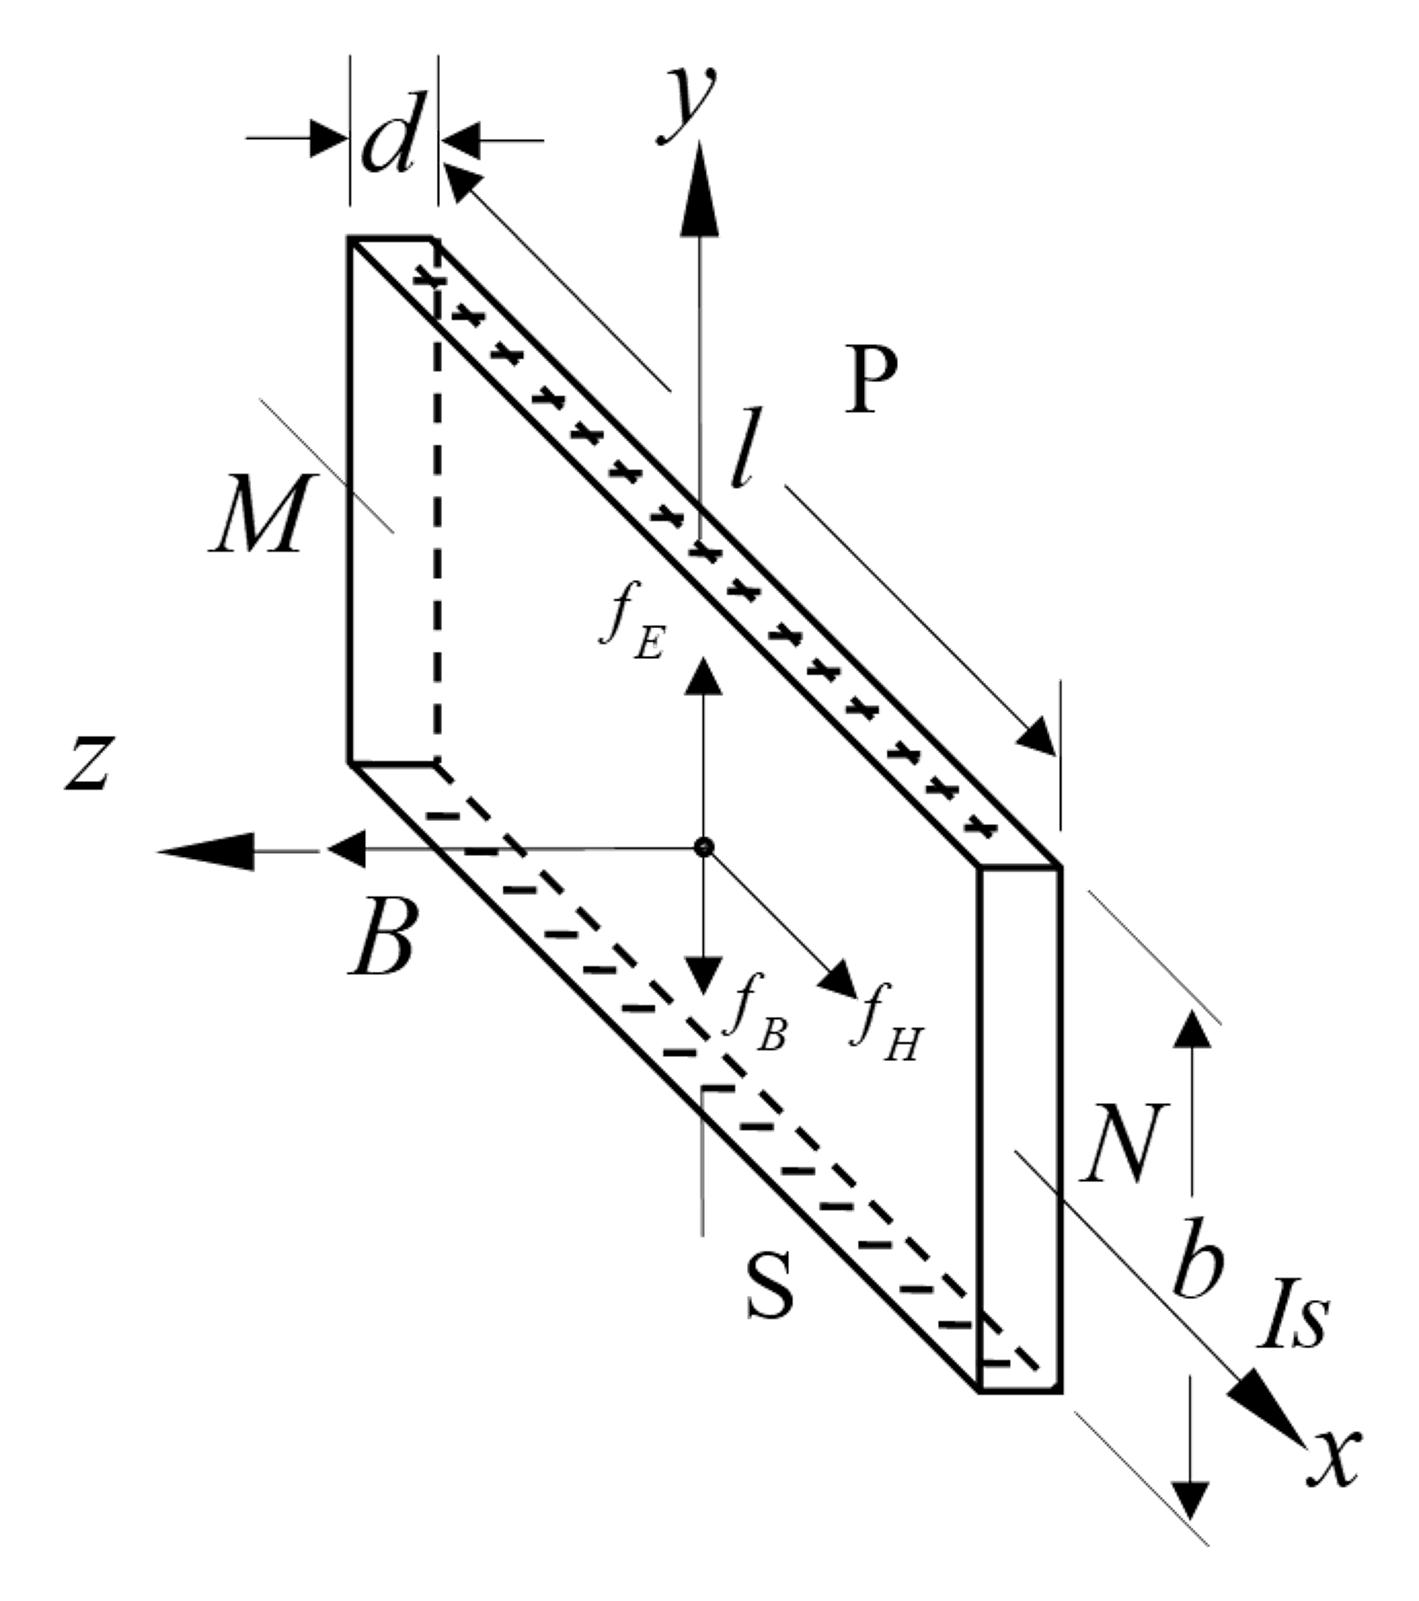
\includegraphics[width=\linewidth]{figures/图1.png}
      \caption{霍尔效应}
    \end{wrapfigure}

    磁场强度测定公式：
    电子受垂直方向磁场$B$的洛伦兹力为$f_B = evB$，电子受侧向电场$E_H$的作用力为$f_E = eE_H$。
    \[
    \begin{aligned}
        \text{稳态时}\quad
        & eE_H = evB,
          \qquad I_s = nevbd
        \\[0.8em]
        \text{所以}\quad
        & V_H = E_H b
          = \frac{1}{ne}\frac{I_s B}{d}
          = R_H \frac{I_s B}{d}
        \\[0.8em]
        \text{设}\quad
        & V_H = K_H I_s B
        \\[0.8em]
        \text{则}\quad
        & B = \frac{V_H}{K_H I_s}
    \end{aligned}
    \]

    载流圆线圈磁场分布：设半径为\(R\)、通有直流电流\(I\)的圆线圈，其轴线上距圆线圈中心\(O'\)为\(X\)处的磁感应强度为
    \[
      B
      =
      \frac{\mu_0 N_0 I R^2}
      {2\left(R^2+X^2\right)^{3/2}}
    \]
    
    其中，\(N_0\)为圆线圈的匝数，\(X\)为轴线上某一点到圆心
    \(O'\) 的距离，\(\mu_0\) 为真空磁导率，其数值为
    \[
        \mu_0 = 4\pi \times 10^{-7}\ \mathrm{H/m}
    \]
    
    载流圆线圈轴线上磁场的分布如图2所示，该磁场分布曲线是一条关于\(Y\)轴对称的单峰曲线。
    
    亥姆霍兹线圈磁场分布：亥姆霍兹线圈的特点是能在其公共轴线中点附近产生均匀磁场区域，如图3所示。

    \begin{figure}[H]
      \centering
      \begin{minipage}{0.4\textwidth}
        \centering
        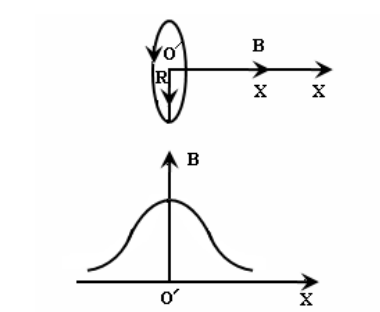
\includegraphics[width=\linewidth]{figures/图2.png}
        \caption{载流圆线圈磁场分布}
      \end{minipage}
      \hfill
      \begin{minipage}{0.4\textwidth}
        \centering
        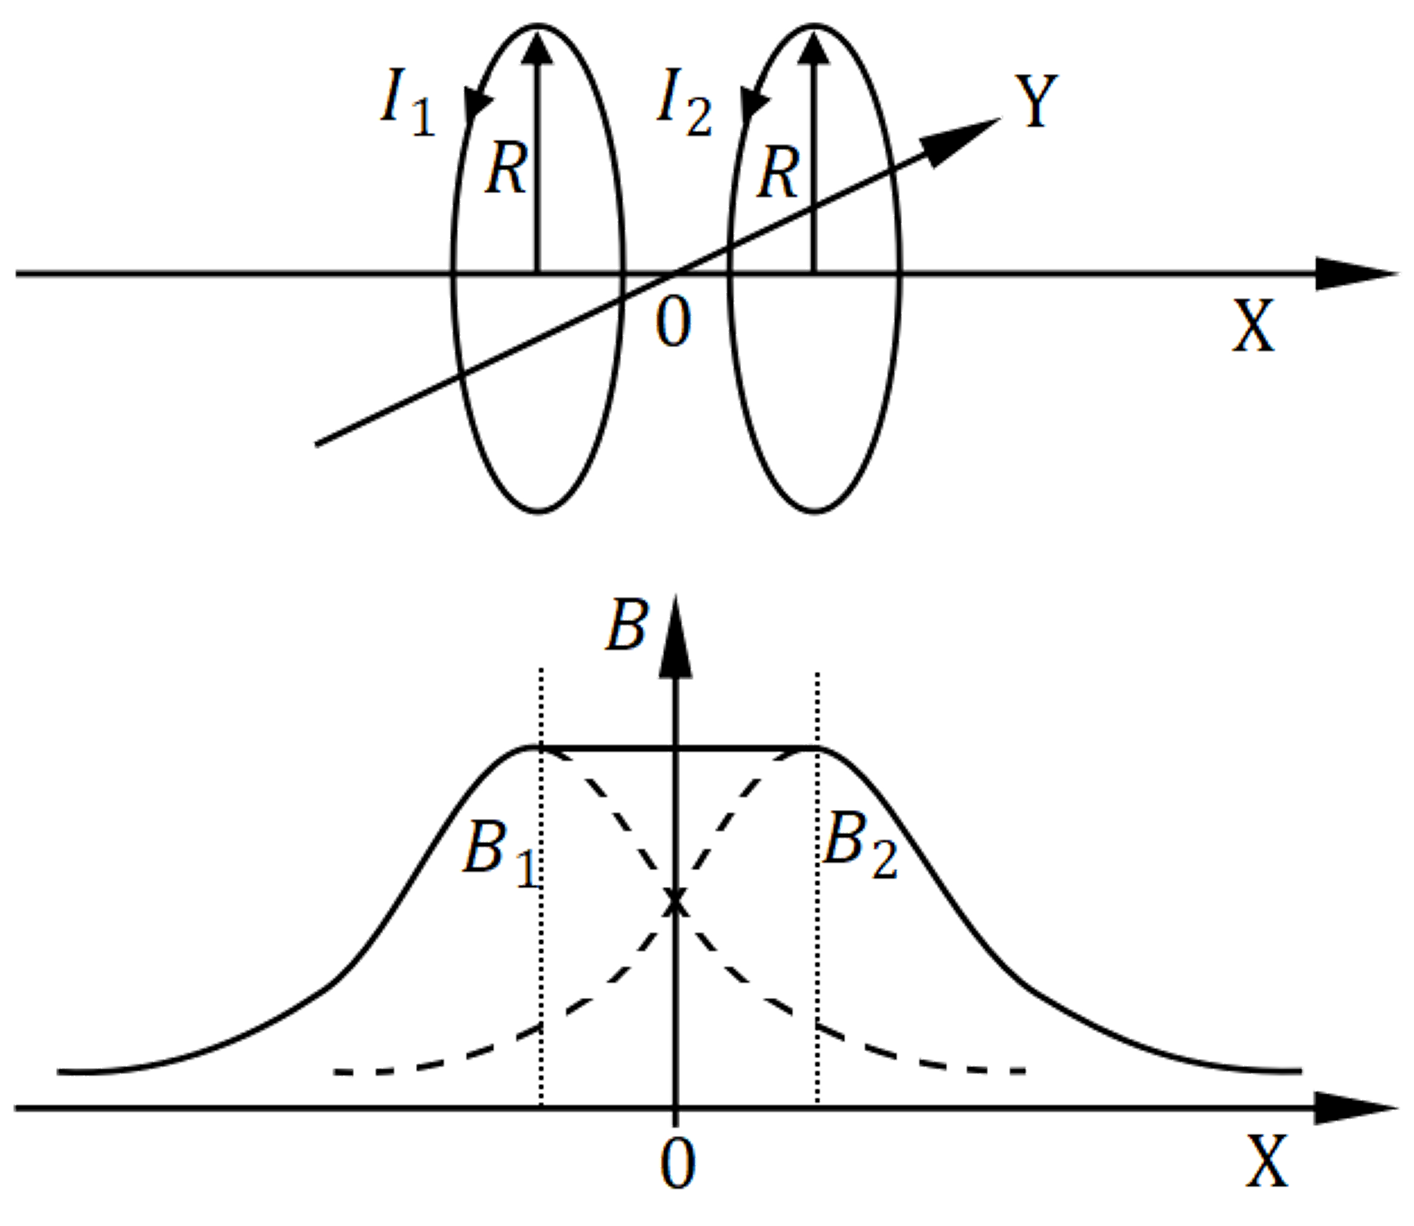
\includegraphics[width=\linewidth]{figures/图3.png}
        \caption{亥姆霍兹线圈磁场分布}
      \end{minipage}
    \end{figure}

  \subsection{实验重点（3分）}
  \begin{enumerate}
    \item 了解霍尔效应基本原理和工作特性；
    \item 测定亥姆霍兹线圈磁场分布；
    \item 掌握磁场测量方法。
  \end{enumerate}
  
  \subsection{实验难点（2分）}
  \begin{enumerate}
    \item 准确定位霍尔探头，使其敏感面垂直于磁场方向；
    \item 保持励磁电流与霍尔工作电流稳定，减小零点漂移和读数误差；
    \item 准确控制测点位置与间距，测量并比较圆线圈与亥姆霍兹线圈的磁场分布。
  \end{enumerate}

\section{实验操作与原始数据（50分）}
% 填写自己的实验数据图

\section{结果与分析（30分）}

  \subsection{数据处理与结果（20分）} 
  单个载流圆线圈和亥姆霍兹线圈的理论磁感应强度可分别按以下公式计算：

  对于单个载流圆线圈，其轴线上距线圈中心$X$处的磁感应强度为
  \[
    B
    =
    \frac{\mu_0 N_0 I R^2}
    {2\left(R^2+X^2\right)^{3/2}}
  \]
  
  其中，$\mu_0$为真空磁导率，$N_0$为线圈匝数，$I$为线圈中的电流，
  $R$为线圈半径，$X$为测量点到线圈中心的轴向距离。
  本实验中，$N_0=400$，$I=400\ \mathrm{mA}$，$R=0.1\ \mathrm{m}$。

  对于亥姆霍兹线圈，设两个完全相同的圆线圈共轴放置，线圈中心间距为$d$，
  测量点到两线圈中点的距离为$X$，则轴线上的磁感应强度为
  \[
    B_{\mathrm{H}}
    =
    \frac{\mu_0 N_0 I R^2}{2}
    \left[
        \frac{1}
        {\left(R^2+\left(X-\dfrac{d}{2}\right)^2\right)^{3/2}}
        +
        \frac{1}
        {\left(R^2+\left(X+\dfrac{d}{2}\right)^2\right)^{3/2}}
    \right]
  \]
  
  其中，$d$为两个线圈的中心间距。

  为比较实验结果与理论计算结果之间的差异，定义平均实验磁感应强度
  $B$与理论磁感应强度$B_{\text{理}}$之间的绝对误差为
  \[
    \Delta B
    =
    \left|B-B_{\text{理}}\right|
  \]

  其中，平均实验磁感应强度可由正向测量值和反向测量值计算得到（若没有测反向则采取正向为平均值）：
  \[
    B
    =
    \frac{\left|B_{\text{正}}\right|
    +\left|B_{\text{反}}\right|}{2}
  \]

  为了消除不同测量点理论磁场大小不同所带来的影响，采用相对误差评价实验结果：
  \[
    \delta_B
    =
    \frac{\left|B-B_{\text{理}}\right|}
    {\left|B_{\text{理}}\right|}
    \times 100\%
  \]
  
  采用上述公式计算得到以下数据表格：

  \begin{table}[H]
    \centering
    \caption{载流圆线圈轴向磁场分布}
    \scriptsize
    \setlength{\tabcolsep}{2.2pt}
    \resizebox{\linewidth}{!}{%
    \begin{tabular}{c*{21}{c}}
      \toprule
      传感器所在位置（cm）
      & 5.00 & 6.00 & 7.00 & 8.00 & 9.00 & 10.00
      & 11.00 & 12.00 & 13.00 & 14.00 & 15.00
      & 16.00 & 17.00 & 18.00 & 19.00 & 20.00
      & 21.00 & 22.00 & 23.00 & 24.00 & 25.00 \\
      \midrule
      轴向距离$x$（cm）
      & -10.00 & -9.00 & -8.00 & -7.00 & -6.00 & -5.00
      & -4.00 & -3.00 & -2.00 & -1.00 & 0.00
      & 1.00 & 2.00 & 3.00 & 4.00 & 5.00
      & 6.00 & 7.00 & 8.00 & 9.00 & 10.00 \\

      正向磁感应强度$B_{\text{正}}$（$\mu\mathrm{T}$）
      & 368 & 428 & 496 & 572 & 652 & 736
      & 825 & 903 & 959 & 997 & 1004
      & 982 & 935 & 868 & 787 & 702
      & 619 & 538 & 469 & 400 & 347 \\

      反向磁感应强度$B_{\text{反}}$（$\mu\mathrm{T}$）
      & -372 & -431 & -498 & -579 & -657 & -741
      & -825 & -902 & -960 & -996 & -1006
      & -984 & -938 & -872 & -790 & -709
      & -622 & -543 & -471 & -407 & -349 \\

      平均磁感应强度$B$（$\mu\mathrm{T}$）
      & 370.0 & 429.5 & 497.0 & 575.5 & 654.5 & 738.5
      & 825.0 & 902.5 & 959.5 & 996.5 & 1005.0
      & 983.0 & 936.5 & 870.0 & 788.5 & 705.5
      & 620.5 & 540.5 & 470.0 & 403.5 & 348.0 \\

      理论磁感应强度$B_{\text{理}}$（$\mu\mathrm{T}$）
      & 355.4 & 412.8 & 478.7 & 552.7 & 633.9 & 719.3 
      & 804.7 & 883.4 & 947.9 & 990.4 & 1005.3 
      & 990.4 & 947.9 & 883.4 & 804.7 & 719.3 
      & 633.9 & 552.7 & 478.7 & 412.8 & 355.4 \\ 

      相对误差（\%）
      & 4.10 & 4.04 & 3.83 & 4.12 & 3.26 & 2.66 
      & 2.53 & 2.16 & 1.23 & 0.61 & 0.03 
      & 0.75 & 1.20 & 1.52 & 2.01 & 1.92 
      & 2.11 & 2.21 & 1.81 & 2.26 & 2.09 \\
      \bottomrule
    \end{tabular}%
    }
  \end{table}

  \begin{table}[H]
    \centering
    \caption{载流圆线圈径向磁场分布}
    \scriptsize
    \setlength{\tabcolsep}{2.5pt}
    \resizebox{\linewidth}{!}{%
    \begin{tabular}{c*{11}{c}}
      \toprule
      径向距离 $x$（cm）
      & -5.00 & -4.00 & -3.00 & -2.00 & -1.00
      & 0.00 & 1.00 & 2.00 & 3.00 & 4.00 & 5.00 \\
      \midrule
      正向磁感应强度$B_{\text{正}}$（$\mu\mathrm{T}$）
      & 1241 & 1136 & 1077 & 1030 & 1010
      & 1001 & 1010 & 1035 & 1075 & 1138 & 1242 \\

      反向磁感应强度$B_{\text{反}}$（$\mu\mathrm{T}$）
      & -1249 & -1145 & -1082 & -1036 & -1015
      & -1008 & -1020 & -1039 & -1081 & -1141 & -1250 \\

      平均磁感应强度$B$（$\mu\mathrm{T}$）
      & 1245.0 & 1140.5 & 1079.5 & 1033.0 & 1012.5
      & 1009.0 & 1015.0 & 1037.0 & 1078.0 & 1139.5 & 1246.0 \\
      \bottomrule
    \end{tabular}%
    }
  \end{table}

  \begin{table}[H]
    \centering
    \caption{亥姆霍兹线圈轴向磁场强度分布（d=R）}
    \scriptsize
    \setlength{\tabcolsep}{2.2pt}
    \resizebox{\linewidth}{!}{%
    \begin{tabular}{c*{21}{c}}
      \toprule
      传感器所在位置（cm）
      & 5.00 & 6.00 & 7.00 & 8.00 & 9.00 & 10.00
      & 11.00 & 12.00 & 13.00 & 14.00 & 15.00
      & 16.00 & 17.00 & 18.00 & 19.00 & 20.00
      & 21.00 & 22.00 & 23.00 & 24.00 & 25.00 \\
      \midrule
      轴向距离$x$（cm）
      & -10.00 & -9.00 & -8.00 & -7.00 & -6.00 & -5.00
      & -4.00 & -3.00 & -2.00 & -1.00 & 0.00
      & 1.00 & 2.00 & 3.00 & 4.00 & 5.00
      & 6.00 & 7.00 & 8.00 & 9.00 & 10.00 \\

      正向磁感应强度$B_{\text{正}}$（$\mu\mathrm{T}$）
      & 880 & 990 & 1103 & 1204 & 1291 & 1360
      & 1410 & 1432 & 1448 & 1455 & 1455 
      & 1453 & 1446 & 1437 & 1410 & 1364 
      & 1295 & 1209 & 1104 & 999 & 886 \\

      反向磁感应强度$B_{\text{反}}$（$\mu\mathrm{T}$）
      & -885 & -1000 & -1105 & -1213 & -1297 & -1364
      & -1412 & -1436 & -1451 & -1453 & -1457
      & -1456 & -1453 & -1442 & -1417 & -1373
      & -1299 & -1218 & -1112 & -1004 & -894 \\

      平均磁感应强度$B$（$\mu\mathrm{T}$）
      & 882.5 & 995.0 & 1104.0 & 1208.5 & 1294.0 & 1362.0
      & 1411.0 & 1434.0 & 1449.5 & 1454.0 & 1456.0
      & 1454.5 & 1449.5 & 1439.5 & 1413.5 & 1368.5
      & 1297.0 & 1213.5 & 1108.0 & 1001.5 & 890.0 \\

      理论磁感应强度$B_{\text{理}}$（$\mu\mathrm{T}$）
      & 890.9 & 1002.1 & 1111.3 & 1211.6 & 1296.4 & 1360.7
      & 1403.3 & 1426.5 & 1436.1 & 1438.5 & 1438.7
      & 1438.5 & 1436.1 & 1426.5 & 1403.3 & 1360.7
      & 1296.4 & 1211.6 & 1111.3 & 1002.1 & 890.9 \\

      相对误差（\%）
      & 0.95 & 0.71 & 0.65 & 0.26 & 0.19 & 0.09
      & 0.55 & 0.52 & 0.93 & 1.08 & 1.20
      & 1.11 & 0.93 & 0.91 & 0.73 & 0.57
      & 0.05 & 0.15 & 0.29 & 0.06 & 0.10 \\
      \bottomrule
    \end{tabular}%
    }
  \end{table}

  \begin{table}[H]
    \centering
    \caption{亥姆霍兹线圈轴向磁场强度分布（d=R/2）}
    \scriptsize
    \setlength{\tabcolsep}{2.2pt}
    \resizebox{\linewidth}{!}{%
    \begin{tabular}{c*{21}{c}}
      \toprule
      传感器所在位置（cm）
      & 5.00 & 6.00 & 7.00 & 8.00 & 9.00 & 10.00
      & 11.00 & 12.00 & 13.00 & 14.00 & 15.00
      & 16.00 & 17.00 & 18.00 & 19.00 & 20.00
      & 21.00 & 22.00 & 23.00 & 24.00 & 25.00 \\
      \midrule
      轴向距离$x$（cm）
      & -10.00 & -9.00 & -8.00 & -7.00 & -6.00 & -5.00
      & -4.00 & -3.00 & -2.00 & -1.00 & 0.00
      & 1.00 & 2.00 & 3.00 & 4.00 & 5.00
      & 6.00 & 7.00 & 8.00 & 9.00 & 10.00 \\

      正向磁感应强度$B_{\text{正}}$（$\mu\mathrm{T}$）
      & 756 & 872 & 1005 & 1145 & 1284 & 1424
      & 1553 & 1670 & 1755 & 1806 & 1824
      & 1804 & 1753 & 1659 & 1556 & 1427
      & 1284 & 1140 & 1001 & 876 & 764 \\

      平均磁感应强度$B$（$\mu\mathrm{T}$）
      & 756 & 872 & 1005 & 1145 & 1284 & 1424
      & 1553 & 1670 & 1755 & 1806 & 1824
      & 1804 & 1753 & 1659 & 1556 & 1427
      & 1284 & 1140 & 1001 & 876 & 764 \\

      理论磁感应强度$B_{\text{理}}$（$\mu\mathrm{T}$）
      & 759.8 & 876.6 & 1006.0 & 1145.5 & 1290.0 & 1432.6
      & 1564.9 & 1677.8 & 1763.9 & 1817.6 & 1835.8
      & 1817.6 & 1763.9 & 1677.8 & 1564.9 & 1432.6
      & 1290.0 & 1145.5 & 1006.0 & 876.6 & 759.8 \\

      相对误差（\%）
      & 0.50 & 0.52 & 0.10 & 0.04 & 0.47 & 0.60
      & 0.76 & 0.47 & 0.51 & 0.64 & 0.65
      & 0.75 & 0.62 & 1.12 & 0.57 & 0.39
      & 0.47 & 0.48 & 0.50 & 0.07 & 0.55 \\
      \bottomrule
    \end{tabular}%
    }
  \end{table}

  \begin{table}[H]
    \centering
    \caption{亥姆霍兹线圈轴向磁场强度分布（d=2R）}
    \scriptsize
    \setlength{\tabcolsep}{2.2pt}
    \resizebox{\linewidth}{!}{%
    \begin{tabular}{c*{21}{c}}
      \toprule
      传感器所在位置（cm）
      & 6.00 & 7.00 & 8.00 & 9.00 & 10.00 & 11.00 
      & 12.00 & 13.00 & 14.00 & 15.00 & 16.00 
      & 17.00 & 18.00 & 19.00 & 20.00 & 21.00 
      & 22.00 & 23.00 & 24.00 & 25.00 & 26.00 \\
      \midrule
      轴向距离$x$（cm）
      & -10.00 & -9.00 & -8.00 & -7.00 & -6.00 & -5.00
      & -4.00 & -3.00 & -2.00 & -1.00 & 0.00
      & 1.00 & 2.00 & 3.00 & 4.00 & 5.00
      & 6.00 & 7.00 & 8.00 & 9.00 & 10.00 \\

      正向磁感应强度$B_{\text{正}}$（$\mu\mathrm{T}$）
      & 1084 & 1081 & 1052 & 1004 & 940 & 880
      & 822 & 770 & 735 & 711 & 705
      & 712 & 739 & 776 & 828 & 895
      & 953 & 1015 & 1064 & 1094 & 1096 \\

      平均磁感应强度$B$（$\mu\mathrm{T}$）
      & 1084 & 1081 & 1052 & 1004 & 940 & 880
      & 822 & 770 & 735 & 711 & 705
      & 712 & 739 & 776 & 828 & 895
      & 953 & 1015 & 1064 & 1094 & 1096 \\

      理论磁感应强度$B_{\text{理}}$（$\mu\mathrm{T}$）
      & 1095.2 & 1092.0 & 1063.0 & 1014.4 & 954.3 & 890.9
      & 831.3 & 780.6 & 742.4 & 718.8 & 710.9
      & 718.8 & 742.4 & 780.6 & 831.3 & 890.9
      & 954.3 & 1014.4 & 1063.0 & 1092.0 & 1095.2 \\

      相对误差（\%）
      & 1.03 & 1.01 & 1.04 & 1.03 & 1.50 & 1.23
      & 1.11 & 1.36 & 1.00 & 1.09 & 0.82
      & 0.95 & 0.46 & 0.59 & 0.39 & 0.46
      & 0.14 & 0.06 & 0.09 & 0.18 & 0.07 \\
      \bottomrule
    \end{tabular}%
    }
  \end{table}

  根据以上数据，绘制成以下$B-x$，$B-y$折线图：

  \begin{figure}[H]
    \centering
    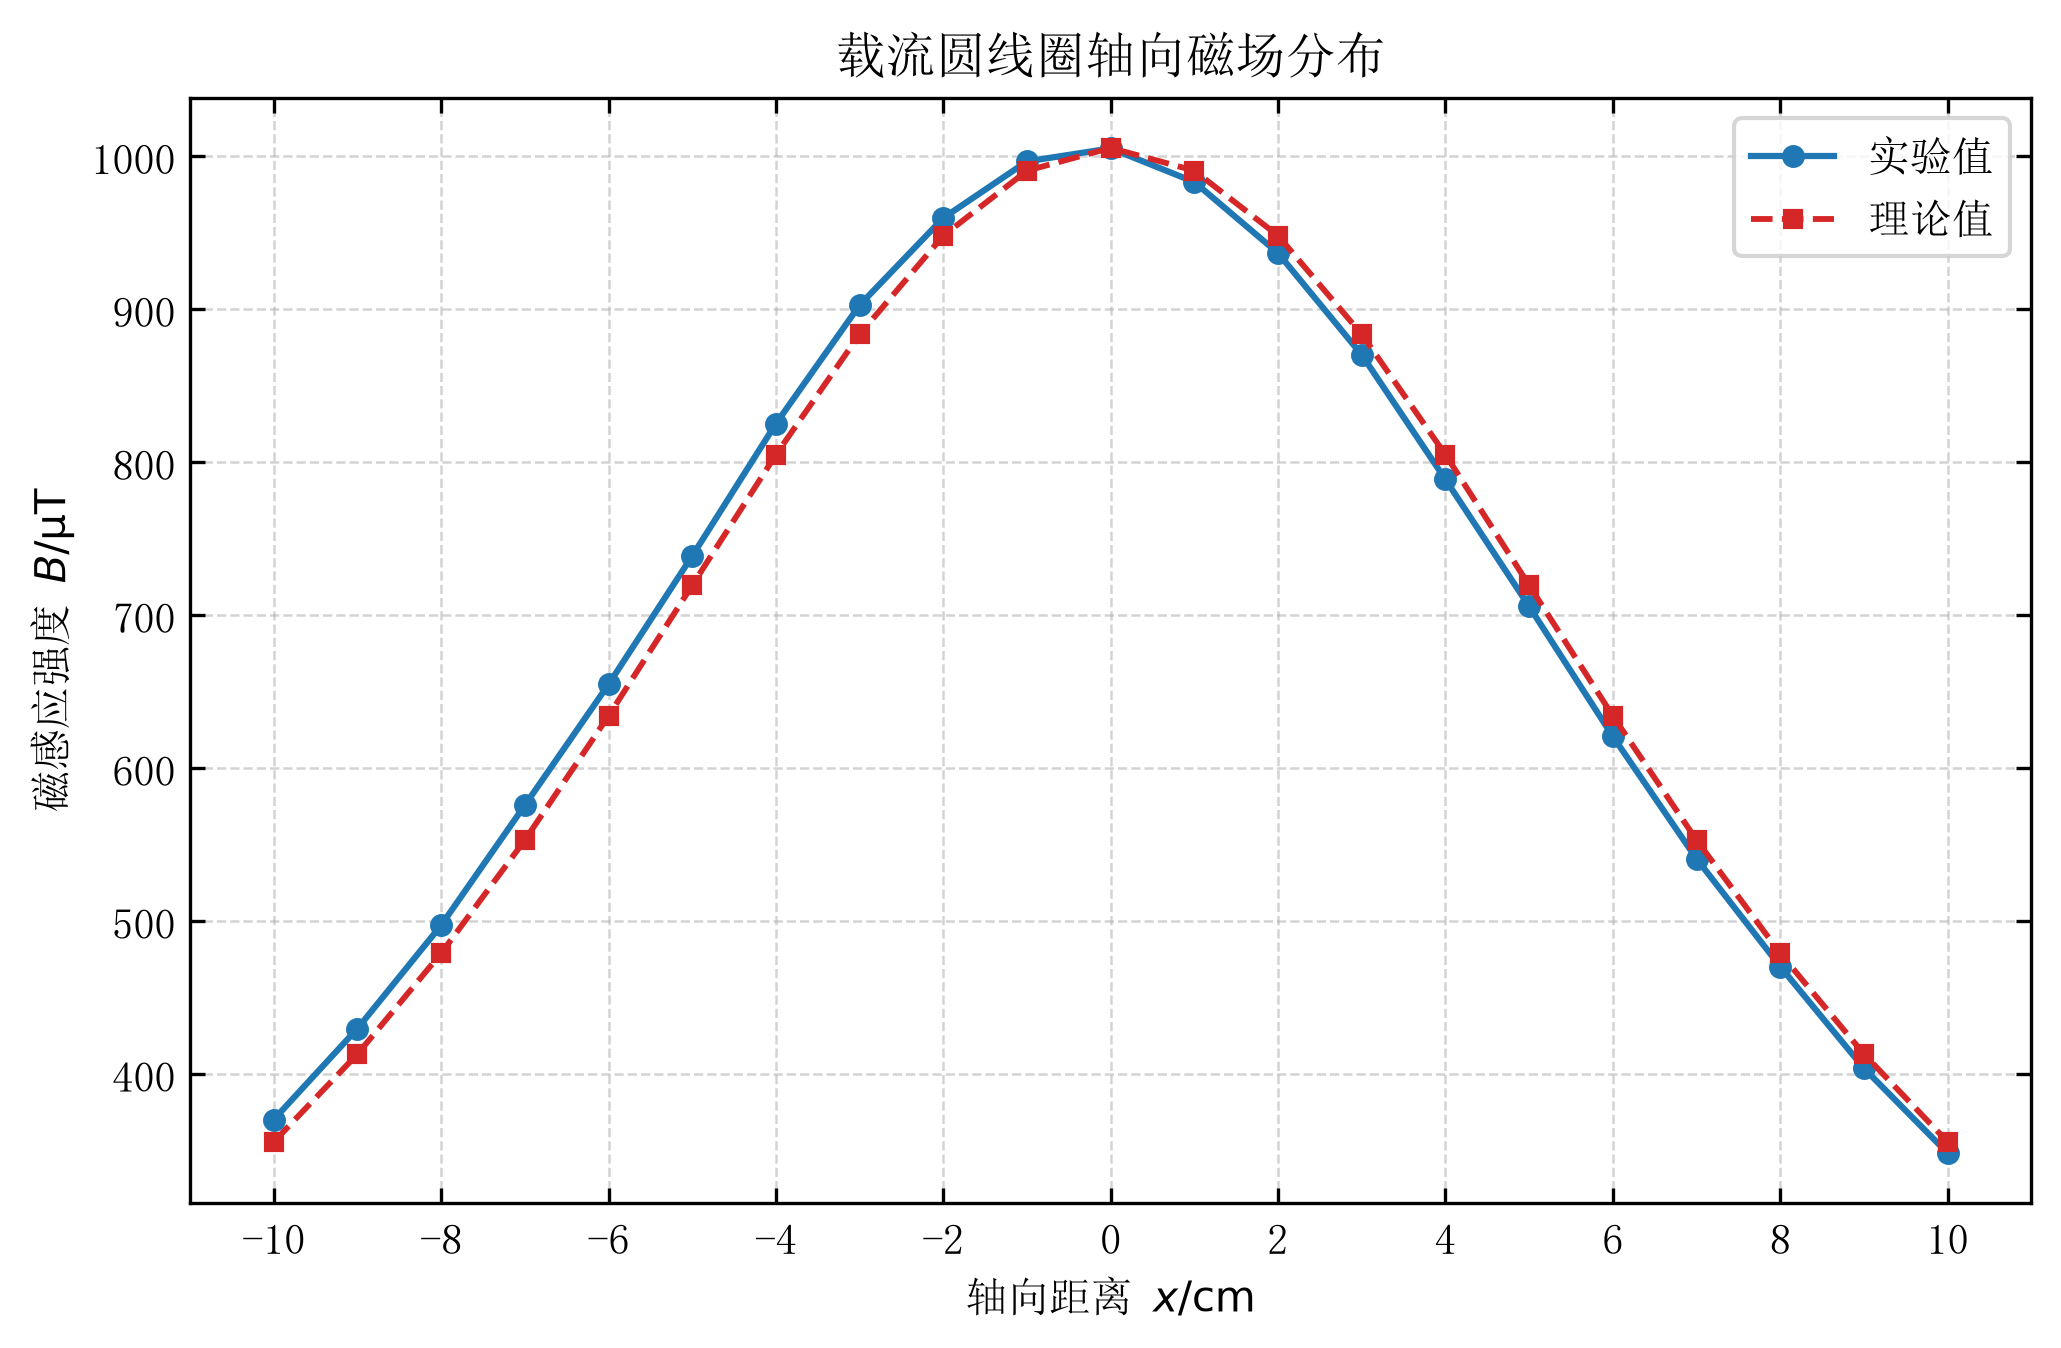
\includegraphics[width=0.65\textwidth]{figures/图6.png}
    \caption{载流圆线圈轴向磁场分布}
  \end{figure}

  \begin{figure}[H]
    \centering
    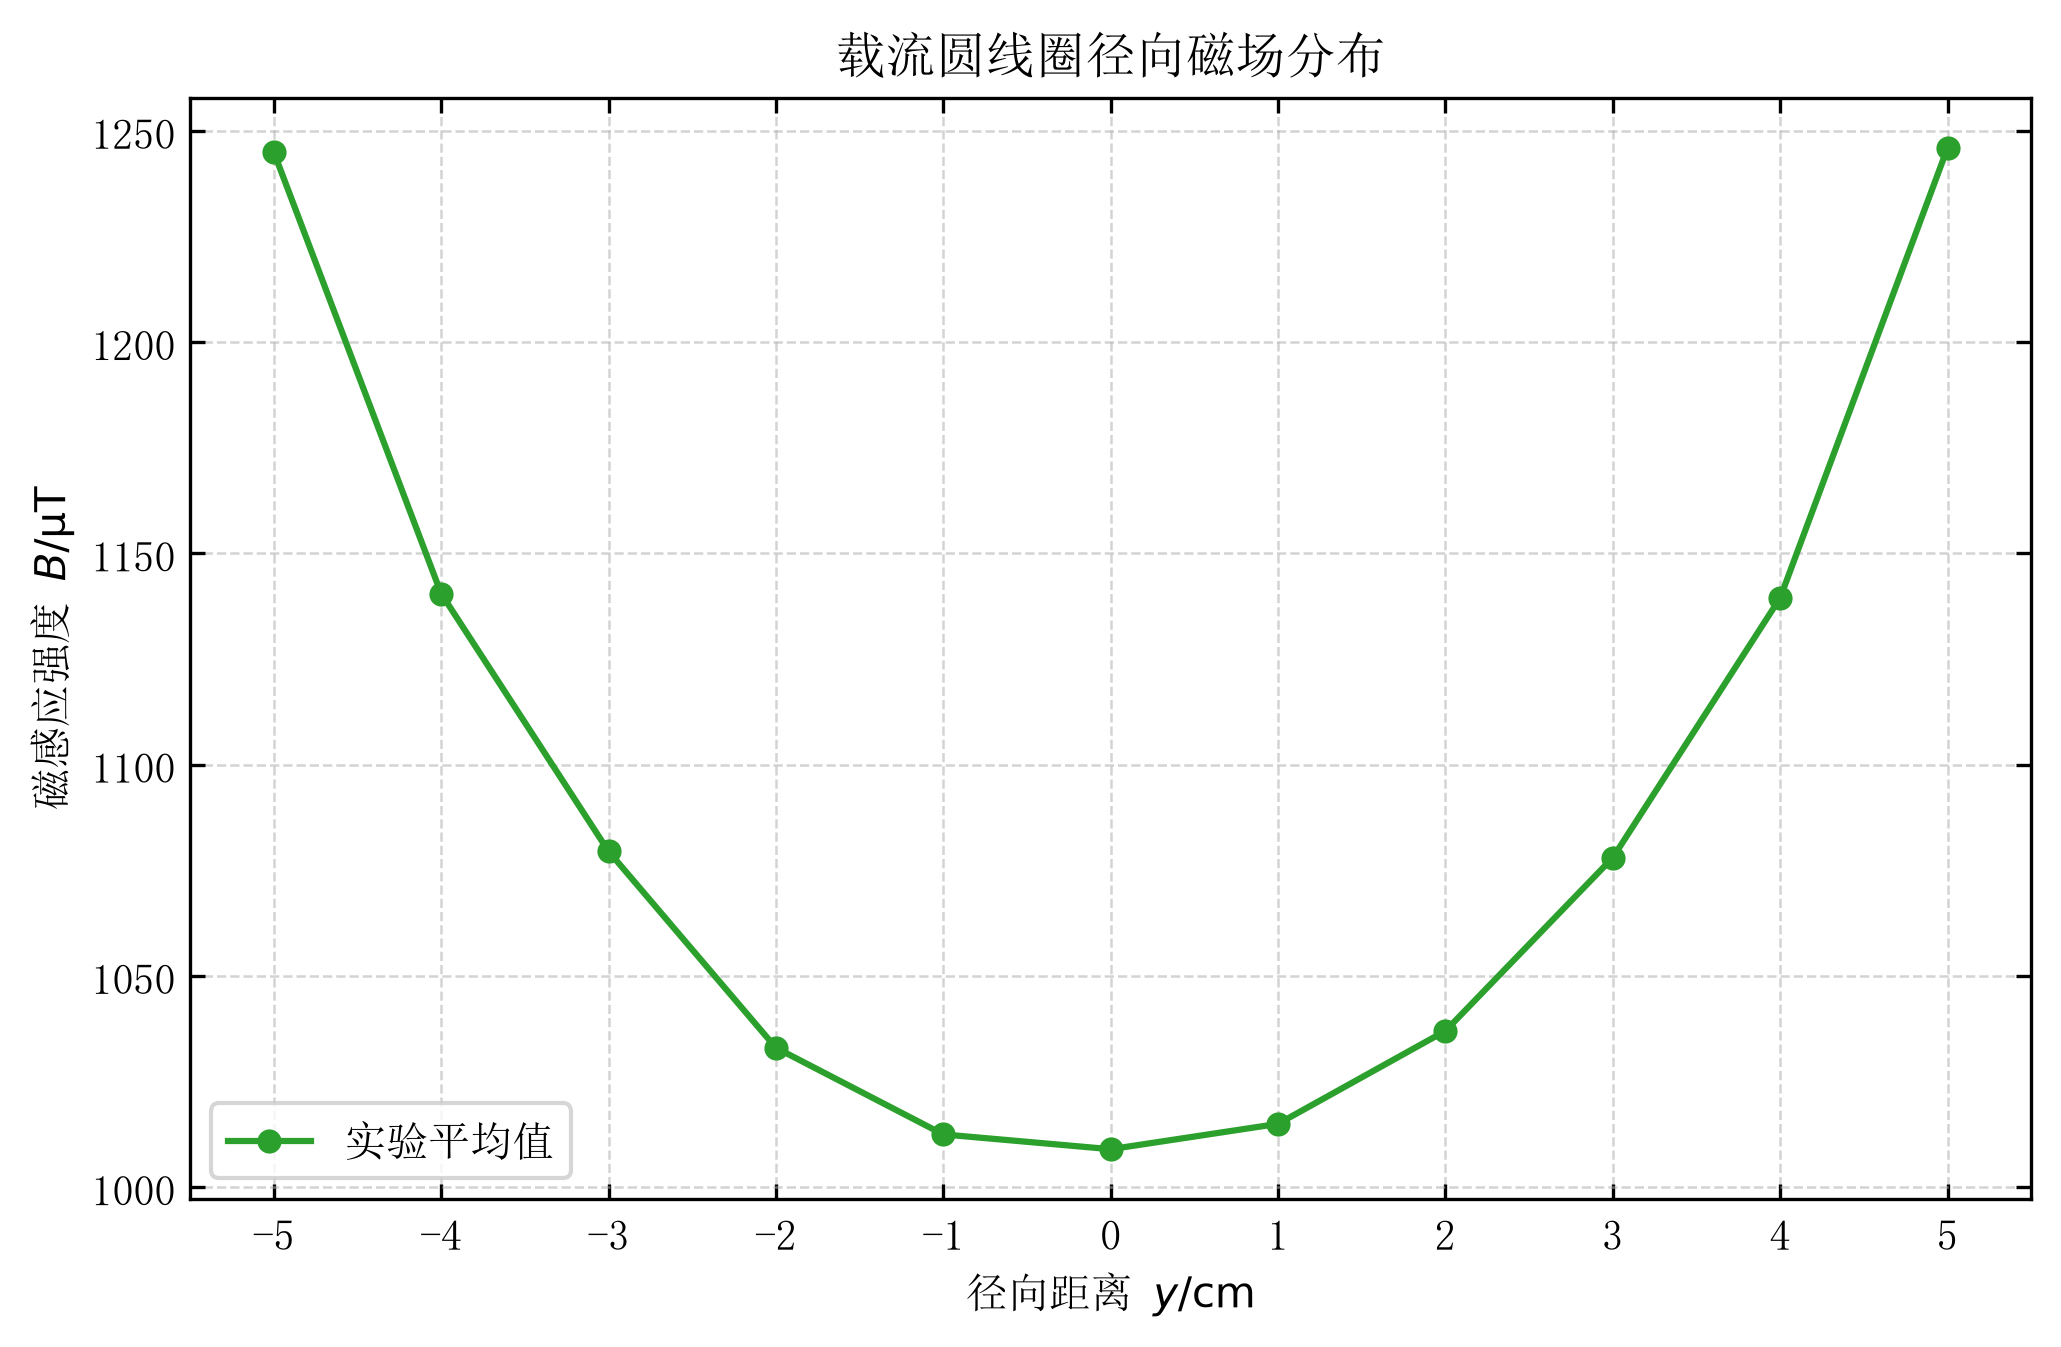
\includegraphics[width=0.65\textwidth]{figures/图7.png}
    \caption{载流圆线圈径向磁场分布}
  \end{figure}

  \begin{figure}[H]
    \centering
    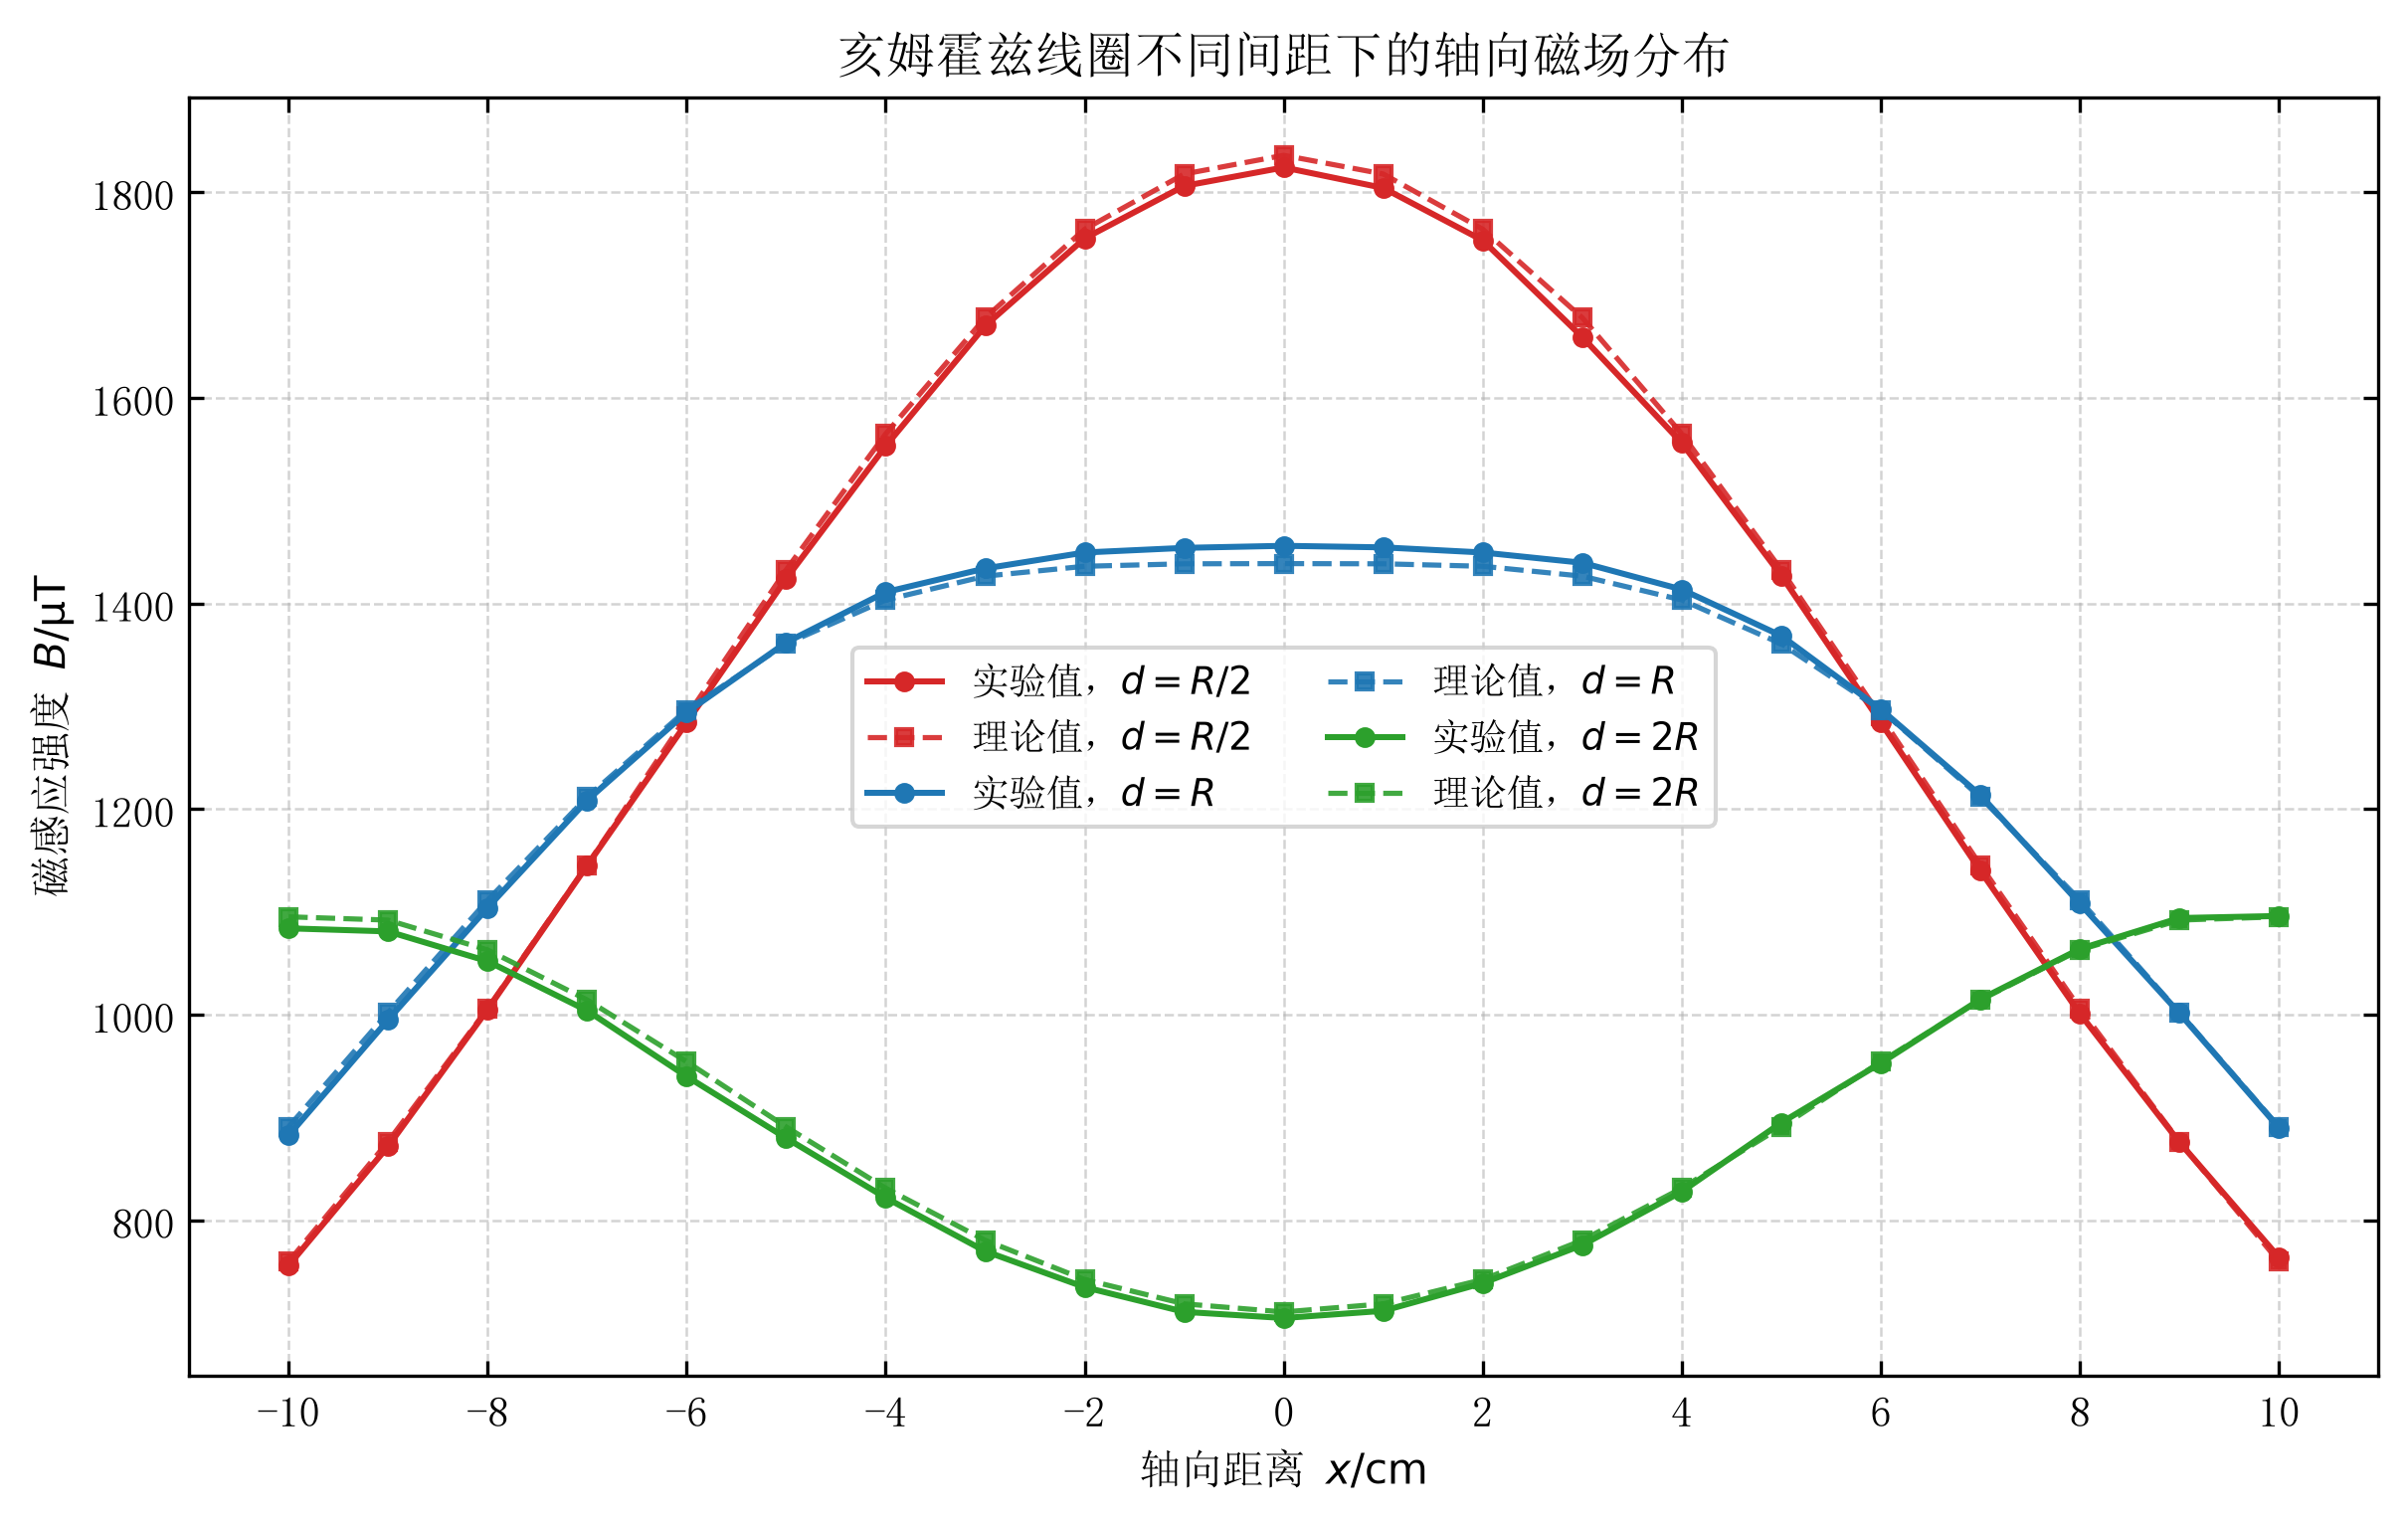
\includegraphics[width=0.65\textwidth]{figures/图8.png}
    \caption{亥姆霍兹线圈不同间距下的轴向磁场分布}
  \end{figure}

  由图6可知，载流圆线圈轴向磁场的实验曲线与理论曲线总体趋势一致，均关于$x=0$附近近似对称。
  在圆线圈中心处，磁感应强度达到最大值，实验值约为$1005.0\,\mu\mathrm{T}$，理论值约为$1005.3\,\mu\mathrm{T}$；随着轴向距离$|x|$逐渐增大，磁感应强度逐渐减小。
  由此可见，单个载流圆线圈轴线上磁场在圆心处最强，远离圆心后磁场强度逐渐衰减。实验曲线与理论曲线在中部区域符合较好，边缘位置有相对明显的偏差，最大相对误差约为$4.13\%$。
  这种偏差可能与霍尔传感器的位置读数误差、线圈实际尺寸与理想模型之间的差异以及环境磁场干扰等因素有关。

  由图7可知，载流圆线圈径向磁场的分布规律与轴向磁场存在明显差异。径向磁感应强度在$y=0$附近达到最小值，实验平均值约为$1009.0\,\mu\mathrm{T}$；
  当传感器沿径向远离圆线圈中心时，磁感应强度逐渐增大，在$y=-5\,\mathrm{cm}$和$y=5\,\mathrm{cm}$处分别约为$1245.0\,\mu\mathrm{T}$和$1246.0\,\mu\mathrm{T}$，
  实验曲线整体呈现出关于$y=0$近似对称的开口向上的变化趋势。
  与轴向方向相比，径向方向上的磁场分布并不是在圆心处最大，而是在远离圆心后逐渐增强。

  由图8可以比较不同线圈间距对亥姆霍兹线圈轴向磁场分布的影响。
  当线圈间距$d=R/2$时，磁场曲线在$x=0$附近呈现较明显的尖峰形状，中心处实验磁感应强度约为$1824\,\mu\mathrm{T}$，为三种间距中最大。
  随着$|x|$增大，磁感应强度较快下降，表明此时磁场主要集中在线圈中部附近，中心区域的均匀性相对较差。

  当线圈间距$d=R$时，磁场曲线在$x=0$附近形成较为平坦的峰顶。中心处实验磁感应强度约为$1456\,\mu\mathrm{T}$，在$x=-2\,\mathrm{cm}$至$x=2\,\mathrm{cm}$范围内，磁感应强度变化较小。
  相比$d=R/2$的情况，虽然中心磁场强度有所降低，但中心区域更加平坦，磁场均匀性明显提高。
  这说明当两线圈间距等于线圈半径时，能够在两线圈中点附近形成较均匀的磁场，体现了亥姆霍兹线圈的主要设计特点。

  当线圈间距$d=2R$时，磁场曲线呈现出与前两种情况不同的凹形分布。
  中心处磁感应强度仅约为$705\,\mu\mathrm{T}$，而在$x=\pm10\,\mathrm{cm}$附近增大到约$1090\,\mu\mathrm{T}$，说明两线圈相距过大时，中点区域的磁场明显减弱，且磁场均匀性变差。
  此时两个线圈产生的磁场在中点附近不能充分叠加，导致中心区域出现磁场低谷。

  综合比较三种线圈间距可知，$d=R/2$时中心磁场强度最大，但磁场曲线变化较快，均匀性较差；$d=R$时中心区域的磁场曲线最为平坦，磁场均匀性最好；$d=2R$时中心磁场强度较小，并且出现明显的凹形分布。
  因此，在实际实验中，若主要目的是获得较均匀的中心磁场，应选择$d=R$的线圈间距；若希望获得较大的中心磁场强度，可以减小线圈间距，但需要牺牲一定的磁场均匀性。

  总体来看，三种不同间距下的实验曲线均能够反映亥姆霍兹线圈磁场随线圈间距变化的基本规律，并与理论分析结果相符得较好。

  \subsection{误差分析（10分）}
  由实验数据及磁场分布曲线可以看出，实验结果的整体变化趋势与理论计算结果基本一致。
  载流圆线圈轴线上的磁感应强度在圆心附近较大，随着测量点远离线圈中心而逐渐减小，且整体分布具有一定的对称性。
  对于亥姆霍兹线圈，两个线圈之间的距离不同，轴线上的磁场分布形状也会有所变化。当线圈间距满足相应条件时，中心附近能够形成较为均匀的磁场区域。

  本实验的误差主要来自以下几个方面：
  \begin{enumerate}
    \item 特斯拉计的仪器误差：霍尔传感器的分辨率、灵敏度和零点稳定性都会影响磁场测量结果。
    实验过程中，仪器读数通常会在发生小幅波动，难以始终稳定在某一个固定值上，会产生一定的随机误差。
    通过正向和反向测量并取平均，可以在一定程度上减小仪器零点偏移的影响。

    \item 传感器位置和方向误差：理论计算要求霍尔传感器准确位于线圈轴线上，并且传感器的敏感方向与磁场方向一致。
    实际移动探头时，很难保证探头始终处于理想位置，位置偏差和角度偏差都会使测得的磁场值发生变化。
    特别是在磁场变化较快的区域，较小的位置偏差也可能造成较明显的读数差异。

    \item 线圈参数和装置结构误差：理论模型通常将线圈视为半径准确、绕制均匀且导线足够细的理想圆线圈。
    实际线圈具有一定的导线直径，绕线分布也不可能完全均匀，线圈的实际半径、匝数以及亥姆霍兹线圈的中心间距都可能与理论取值存在差异。
    这些因素会使得实际磁场分布与理论模型并不完全一致。

    \item 电流波动带来的误差：线圈产生的磁场强度与电流大小有关。
    实验过程中，电源输出可能存在轻微波动，接线电阻和接触情况也可能发生变化，从而使线圈中的实际电流发生变化。

    \item 地磁场和环境杂散磁场的影响：实验室中始终存在地磁场，附近的通电导线、铁磁性物体以及其他实验仪器也可能产生杂散磁场。
    特斯拉计测得的实际结果会受到这些环境磁场的影响，从而使实验数据产生一定偏移。
  \end{enumerate}

  总体来看，本实验得到的磁场分布趋势与理论结果基本一致，说明理论模型能够较好地描述载流圆线圈和亥姆霍兹线圈的磁场分布规律。
  若要进一步提高实验精度，可以增加测量次数，采用固定导轨控制传感器位置，并在测量前后分别进行背景磁场和仪器零点校正。
\section{实验探讨与思考题（10分）}

  \subsection{实验探讨}
  本实验研究了载流圆线圈和亥姆霍兹线圈轴线上的磁场分布规律。
  通过改变传感器的位置，分别测量了不同位置处的磁感应强度，并将实验结果与理论计算值进行了比较。

  对于载流圆线圈，磁感应强度在圆心处达到最大值，随着测量点逐渐远离线圈中心，磁感应强度逐渐减小，整体分布关于线圈中心近似对称。

  对于亥姆霍兹线圈，当两线圈间距满足特定条件时，两个线圈产生的磁场在中间区域相互叠加，使中心附近形成较为均匀的磁场区域。
  实验测量了线圈不同间距下的磁场分布情况，并发现当线圈间距等于线圈半径时，中心区域的磁场最为平坦，均匀性最好；
  而当线圈间距小于或大于线圈半径时，中心区域的磁场分布则出现明显的峰形或凹形特征。

  \subsection{思考题}

    \subsubsection{为什么在测量直流磁场时，必须考虑地球磁场对被测磁场的影响？}
    答：地球本身相当于一个巨大的磁体，实验室中始终存在着一定大小的地磁场。
    测量磁场时，仪器实际测得的是被测磁场与地磁场以及周围环境杂散磁场的矢量叠加，而不是待测线圈单独产生的磁场。
    地磁场的大小虽然通常只有几十微特斯拉，但在测量较弱磁场或比较理论值与实验值时，其影响可能不能忽略。
    若不对地磁场进行修正，测量结果会出现整体偏移，并可能影响磁场分布曲线的对称性和实验误差。

    \subsubsection{亥姆霍兹线圈是怎样组成的？其基本条件有哪些？它的磁场分布特点又怎样？改变两圆线圈间距后，线圈轴线上的磁场分布情况如何？}
    答：亥姆霍兹线圈由两个完全相同的圆形线圈组成。两个线圈具有相同的半径、匝数和电流，线圈共轴且彼此平行，电流方向相同。
    标准亥姆霍兹线圈的两个线圈中心间距通常取为线圈半径，即
    \[
    d=R
    \]

    在满足上述条件时，两个线圈在中间区域产生的磁场方向相同，磁场相互叠加。
    由于结构具有较高的对称性，中点附近磁场的变化较小，因此可以形成较为均匀的磁场区域。在线圈轴线上，磁场分布关于两线圈中点近似对称。

    当线圈间距小于半径，即$d<R$时，中心附近的磁场通常表现为较明显的峰形分布，中心处磁场较大但均匀区域较小。
    当$d=R$时，中心附近的磁场最为平坦，均匀性较好。当线圈间距大于半径，即$d>R$时，中心区域的磁场均匀性变差，轴线上可能出现中间较低、两侧较高的分布特点。

    因此，线圈间距是影响轴线上磁场均匀性的重要因素。标准亥姆霍兹线圈通过选择$d=R$，使中点附近的磁场具有较好的均匀性。

    \subsubsection{霍尔元件放入磁场时，不同方向上的特斯拉计指示值不同，哪个方向最大？}
    答：霍尔元件具有确定的敏感方向，只有磁场在敏感方向上的分量能够有效产生霍尔电压。
    当霍尔元件的敏感轴与磁场方向平行，或者霍尔片平面与磁场方向垂直时，磁场在敏感方向上的分量最大，因此特斯拉计的指示值最大。

    若霍尔元件的敏感方向与磁场方向之间存在夹角 $\theta$，则仪器测得的有效磁场分量可表示为
    \[
    B_{\text{测}}=B\cos\theta
    \]
    当$\theta=0$时，测量值最大；当霍尔元件的敏感方向与磁场方向垂直时，理论上测量值应接近于零。

    因此，测量时应旋转霍尔探头，使其敏感轴尽可能与待测磁场方向一致，以获得最大的读数。

    \subsubsection{自主设计测量地磁场的实验方案}
    答：可以利用霍尔传感器分别测量地磁场在三个相互垂直方向上的分量，再由矢量合成得到地磁场的大小。

    首先，将特斯拉计进行调零，并远离载流线圈、铁磁性物体和大型用电设备，以减小实验室杂散磁场的影响。
    利用指南针确定当地的南北方向，将霍尔探头的敏感轴分别调整到南北方向、东西方向以及竖直方向。

    在每个方向上分别测量一次正向读数和一次反向读数。若仪器能够显示带符号的磁场值，可以采用
    \[
    B_i=\frac{B_i^{+}-B_i^{-}}{2}
    \]
    计算该方向上的地磁场分量；若仪器只显示磁场大小，则可以对正、反两个方向的读数取平均，以减小读数误差和零点偏移的影响。
    分别得到南北方向、东西方向和竖直方向的磁场分量
    $B_x$、$B_y$和$B_z$后，地磁场总强度可由下式计算：
    \[
    B_{\text{地}}
    =
    \sqrt{B_x^2+B_y^2+B_z^2}
    \]

    为了提高测量精度，每个方向可以重复测量多次并取平均值。最后，将测得的地磁场大小与当地地磁场的参考值进行比较，并分析误差来源。

\vspace*{\fill} % 使下面内容在页面底部显示
\noindent
\begin{minipage}{\textwidth}
  注意事项：

  \begingroup
    \setlength{\leftskip}{2em} % 1--4整体向右缩进两个汉字宽度
    1. 用PDF格式上传“实验报告”，文件名：学生姓名+学号+实验名称+周次。

    2. “实验报告”必须递交在“学在浙大”本课程内对应实验项目的“作业”模块内。

    3. “实验报告”成绩必须在“浙江大学物理实验教学中心网站”-“选课系统”内查询。

    4. 教学评价必须在“浙江大学物理实验教学中心网站”-“选课系统”内进行，学生必须进行教学评价，才能看到实验报告成绩，教学评价须在本次实验结束之后3天内进行。\par
  \endgroup

  \begin{center}
    {\CJKfontspec[AutoFakeBold=2.5]{SimSun}\bfseries 浙江大学物理实验教学中心制}
  \end{center}
\end{minipage}

\end{document}
